\section{Specifying Counting Networks in Hoare Style}
\label{sec:counting}

We now show how one can use histories and subjectivity to specify
another class of non-linearizable objects---\emph{counting networks}.

Counting networks are a special case of \emph{balancing networks}
introduced by Aspnes \etal~\cite{Aspnes-al:JACM94}, themselves
building on sorting networks~\cite{Ajtai-al:STOC83}. Counting networks
implement concurrent counters in a way free from synchronization
bottlenecks.
%
The key idea of counting networks is to decompose the workload between
\emph{several} counters, so that each of them is responsible for a
disjoint set of values. A thread trying to perform an incrementation
first approaches the \emph{balancer}, which is a logical ``switch''
that ``directs'' the thread, \ie, provides it with the address of the
counter to increment.
%
The balancers make counting networks' operations
\emph{non-linearizable}, as in the presence of interference the
results of increments might be observed out of order.
%
% \wrt~a sequential specification.

\begin{figure}%[18]{r}{4cm} 
\begin{tabular}{c@{\ \ \ \ \ \ }c}
\begin{minipage}[c]{2.5cm}
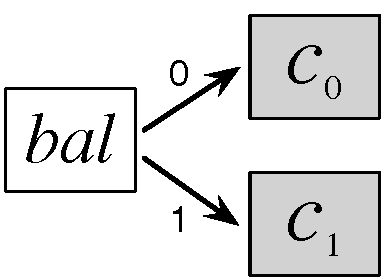
\includegraphics[width=2.1cm]{counter.pdf} 
\end{minipage}
&
\begin{minipage}[l]{4.9cm}
\centering
{\small{
\[
\begin{array}{rl}
\Num{1} & \esc{getAndInc()} : \esc{nat}~=~\esc{\{}  \\[2pt] 
\Num{2} & ~~~~ b \Asgn \esc{flip(}\bal\esc{)};\\[2pt]
\Num{3} & ~~~~ \res \Asgn \esc{fetchAndAdd2(}c_b\esc{)};\\[2pt]
\Num{4} & ~~~~ \kw{return}~\res~\esc{\}}
\end{array}
\]
}}
\end{minipage} 
\\
(a) & (b)
%
\end{tabular}
%
\caption{Simple counting network: intuition and pseudo-code.}
\label{fig:counter-fig} 
\end{figure}

Figure~\ref{fig:counter-fig} presents a schematic outline (a) and a
pseudo-code implementation (b) of a counting network with a single
balancer.
%
The implementation contains three pointers: the balancer $\bal$, which
stores either 0 or 1, thus directing threads to the shared pointers
$c_0$ or $c_1$, which count the even and odd values,
respectively. Threads increment by calling \code{getAndInc}, which
works as follows. It first atomically changes the bit value of the
balancer via a call to atomic operation \code{flip} (line 2). The
\code{flip} operation returns the \emph{previous} value $b$ of the
balancer as a result, thus determining which of the counters, $c_0$ or
$c_1$, should be incremented. The thread proceeds to atomically add 2
to the value of $c_b$ via \code{fetchAndAdd2} (line 3). The old value
of $c_b$ is returned as the result of the procedure.\footnote{In the
  counting network from Figure~\ref{fig:counter-fig}, the balancer
  itself might seem like a contention point. However, the \code{flip}
  operation is much less expensive than \code{CAS} as a
  synchronization mechanism. The performance can be further improved
  by constructing a \emph{diffracting tree} of several
  balancers~\cite[\S 12.6]{Herlihy-Shavit:08}, but we do not consider
  diffracting trees here.}

Assuming that $c_0$ and $c_1$ are initialized with $0$ and $1$, it is
easy to see that in a single-threaded program, the network will behave
as a conventional counter; that is, consecutive invocations of
\code{getAndInc} return consecutive nats.
%
However, in the concurrent setting, \code{getAndInc} may return
results out of order, as follows. 
%
% which historically led to the definition of quiescent
% consistency~\cite[\S 3.3]{Herlihy-Shavit:08} in order to specify the
% network's concurrent behavior.

\vspace{3pt}
\begin{example}
\label{ex:t1t2}
%
Consider two threads, $T_1$ and $T_2$ operating on the network
initialized with $\bal\,{\mapsto}\,0$, $c_b\,{\mapsto}\,b$. $T_1$
calls \code{getAndInc} and executes its line~2 to set $\bal$ to 1. It
gets suspended, so $T_2$ proceeds to execute lines~2 and~3, therefore
setting $\bal$ back to $0$ and returning $1$. While $T_1$ is still
suspended, $T_2$ calls \code{getAndInc} again, gets directed to $c_0$,
and returns 0, after it has just returned 1.
%
\end{example}
\vspace{3pt}

\noindent

This out-of-order behavior, however, is not random, and can be
precisely characterized as a function of the number of threads
operating on the
network~\cite{Afek-al:OPODIS10,Jagadeesan-Riely:ICALP14}. In the rest
of this section and in Section~\ref{sec:qc-client}, we show how to
capture such bounds precisely using auxiliary state of (subjective)
histories in a client-sensitive manner. As a form of road map, we
first list the desired requirements for the spec of \code{getAndInc},
%
adapting the design goals of the criteria, such as QC, QQC and
QL~\cite{Aspnes-al:JACM94,Afek-al:OPODIS10,Jagadeesan-Riely:ICALP14},
which we will proceed to verify formally, and then employ in
client-side reasoning.
%
\vspace{2pt}
\begin{itemize}

\item \textbf{R1:} Two different calls to \code{getAndInc}
  should return distinct results (\emph{strong concurrent
    counter semantics}).

\item \textbf{R2:} The results of calls to \code{getAndInc},
  separated by a period of quiescence (\ie, absence of interference),
  should appear in their sequential order (\emph{quiescent
    consistency}).

\item \textbf{R3:} The results of two sequential calls $C_1$ and
  $C_2$, in a single thread should be out of order by no more than
  $2\ N$, where $N$ is the number of interfering calls that overlap
  with $C_1$ and $C_2$ (\emph{quantitative quiescent
    consistency/quasi-linearizability}).
%\an{Can we chose one of the two here: either qqc or ql?}

\end{itemize}

\begin{comment}
\noindent 
In the rest of this and in the next section, we will illustrate how to
achieve all these goals by employing (a) \emph{subjective auxiliary
  state} as a mechanism for \emph{{explicitly referring to and
    quantifying over}} the effects of currently interfering threads
(via its \emph{other}-component) in combination with (b)
\emph{histories}, providing a way to \emph{{logically record relevant
    pieces of state information}} (including witnessed interference)
in Hoare-style program specifications.
\end{comment}

%\vspace{2pt}
%\lipsum[1]

\subsection{Formalizing the counting network}
\label{sec:counting-intuition}

To formalize the necessary invariants, we elaborate the counting
network with auxiliary state: \emph{tokens} (isomorphic to nats) and
\emph{interference-capturing histories}.

A \emph{token} provides a thread that owns it with the right to
increment an appropriate counter~\cite{Aspnes-al:JACM94}. In our
example, a thread that performs the \code{flip} in line 2 of
\code{getAndInc} will be awarded a token which it can then spend to
execute \code{fetchAndAdd2}.
%
Thus, any individual token represents a ``pending'' call to
\code{getAndInc}, and the set of unspent tokens serves as a bound on
the out-of-order behavior that the network exhibits. We will have four
different auxiliary variables tracking the different classes of
tokens: $\tkns^0$ and $\tkns^1$ keep the tokens owned by the
\emph{self} thread, administering access to $c_0$ and $c_1$,
respectively. Similarly, $\tkno^0$ and $\tkno^1$ keep the tokens owned
by the \emph{other} thread. We abbreviate $\tkn^i = \tkns^i \hunion
\tkno^i$, $i=0,1$, $\tkns = \tkns^0 \hunion \tkns^1$, $\tkno = \tkno^0
\hunion \tkno^1$.

Figure~\ref{fig:chist} illustrates a network with three \emph{even}
tokens: $x^0, y^0, z^0 \in \tkn^0$, held by threads that will
increment $c_0$, and one \emph{odd} token $u^1 \in \tkn^1$, whose
owner will increment $c_1$.
%
%\an{Removed: We also point out here that token names (and their
%  uniqueness) will be of critical importance for the specifications we
%  give further. This point was never emphasized later on, so why
%  bother drawing attention to it.}

\begin{figure}
\centering
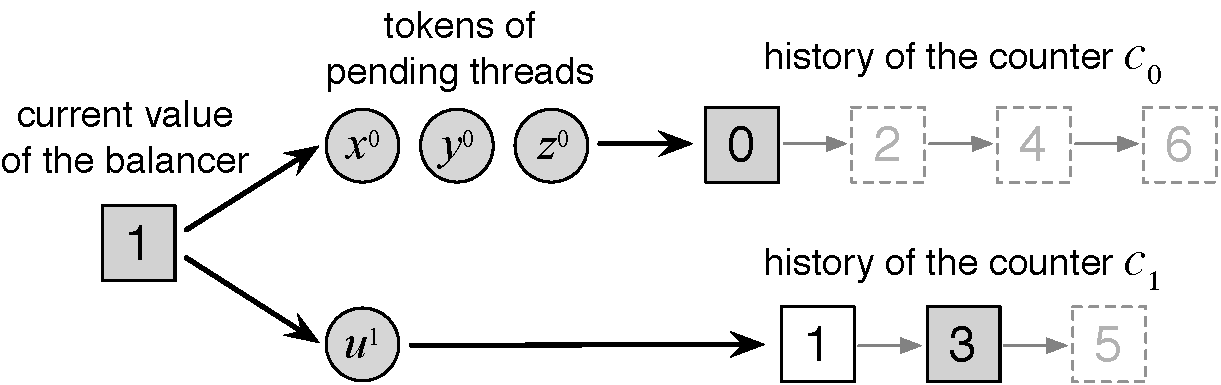
\includegraphics[width=8.2cm]{chist.pdf}      
\caption{Tokens and histories of the simple counting network.}
\label{fig:chist}
\end{figure}

A \emph{history} of the counting network is an auxiliary finite map,
consisting of entries of the form
\[
\tag{\normalsize{\arabic{tags}}}\refstepcounter{tags}\label{eq:cn-entry} 
%
t \mapsto (\tknh^0, \tknh^1, z)
\]
Such an entry records that the value $t$ has been written into an
appropriate counter ($c_0$ or $c_1$, depending on the parity of $t$),
at the moment when $\tkn^0$ and $\tkn^1$ held values $\tknh^0$ and
$\tknh^1$, respectively. Moreover, in order to write $t$ into a
counter, the token $z$ was spent by the thread invoking
\code{getAndInc}. We will refer to $z$ as the \emph{spent}
token. Notice that the entries in the history contain tokens held by
both \emph{self} and \emph{other} threads. Thus, a history captures
the behavior of a thread subjectively, \ie, as a function of the
behavior of the threads interfering with it.

Similarly to tokens, network histories are split into four different
auxiliary variables, which are manipulated differently by our
proofs. Thus, we have $\hists^0$ and $\hists^1$ to track the even and
odd counter updates performed by the \emph{self} thread, and dually
$\histo^0$ and $\histo^1$ for the \emph{other} thread. We abbreviate
$\hist^i = \hists^i \hunion \histo^i$, $i = 0,1$, and $\hists =
\hists^0 \hunion \hists^1$, and $\histo = \histo^0 \hunion \histo^1$.

Figure~\ref{fig:chist} illustrates a moment in network's history and
how it relates to the state of the counters. Only $0$ has been written
to $c_0$ so far (upon initialization), hence $\hist^0$ only contains
an entry for $t = 0$ (we ignore at the moment the \emph{contents} of
the history entries). On the other hand, $\hist^1$ has entries for $1$
and $3$, because after initialization, one thread has increased $c_1$.
%
The gray boxes indicate that $0$ and $3$ are the current values of
$c_0$ and $c_1$, and thus also the latest entries in $\hist^0$ and
$\hist^1$, respectively. In particular, these values will be returned
by the next invocations of \code{fetchAndAdd2}. The dashed boxes
correspond to the entries to be added to the history by the currently
running threads holding the tokens $x^0$, $y^0$, $z^0$,
$u^1$. However, as thread scheduling is non-deterministic, we cannot
predict which of the tokens will be spent to, say, write 2 into $c_0$
(it may be any of the even tokens). On the other hand, in the absence
of other threads joining the network, we know that token $u^1$ will be
spent to write $5$ into $c_1$.

\subsubsection{Resource invariants of the counting network}
\label{sec:count-netw-invar}
We next formally list the invariants that describe the interdependence
between the various components of the real and auxiliary state. In
addition to $\tkn$ and $\hist$ which come in flavors private to
\emph{self} and \emph{other} threads, we require the following joint
variables: (1) $\heapj$ which stands for the joint heap of the
network, and (2) $b_\joint$, $n^0_\joint$ and $n^1_\joint$ which stand
for the contents of $\bal$, $c_o$ and $c_1$, respectively. 

The main invariant of the network relates the number of tokens, the
size of histories and the value of the balancer as follows.
%
\[
\tag{\normalsize{\arabic{tags}}}\refstepcounter{tags}\label{cn:si} 
%
|\hist^0| + |\tkn^0| =
|\hist^1| + |\tkn^1| + b_\joint
\]
%
The equation directly motivates our design of the auxiliary state, and
leads to establishing the requirements \textbf{R1}--\textbf{R3}. It
formalizes the intuition that out-of-order anomalies of the counting
network appear if one of the two counters is too far ahead of the
other one.
%
The invariant~(\ref{cn:si}) provides a bound on such a situation. One
counter can get ahead temporarily, but then the other counter must
have a number of threads waiting to spend their tokens, and increment
it. Thus, the other counter will eventually catch up.

The approaches such as quiescent and quantitative quiescent
consistency describe this situation by referring to the number of
\emph{unmatched} call events in an event
history~\cite{Derrick-al:FM14,Jagadeesan-Riely:ICALP14}. In contrast,
we formalize this property by relying on auxiliary state. In our case,
the sets of tokens $\tknh^0$ and $\tknh^1$ recorded in the entry for
the number $t$ determine the environment's capability to add new
history entries, and thus ``run ahead'' or ``catch up'' after $t$ has
been returned. Such auxiliary state will let us directly specify the
network's behavior in the moments of quiescence (\ie,~when $\tkno$ is
empty), but also \emph{quantitatively} bound the out-of-orderness as a
function of $\tkno$.

We next list the other resource invariants.
\vspace{2pt}
\begin{enumerate}[label=(\roman*)]

% %
% \[
% \tag{\normalsize{\arabic{tags}}}\refstepcounter{tags}\label{eq:cn-states} 
% {\small
% \begin{array}{r@{\ }c@{\ }l} 
% {\!\!\!\!\!\!\!\!}W_{\ccon} & \!\eqdef & \exists \tkns~\tkno~ \hists~\histo~b~n_0~n_1\ldot 
% %  
% \qcl \spts (\tkns, \hists)\aand \qcl \opts (\tkno, \histo) 
%   \\[4pt] 
% &\aand & \qcl \jpts \bal \hpts b \hunion c_0 \hpts n_0 \hunion c_1 \hpts n_1   
%  \aand \hvalid~(\hists \hunion \histo)         \\[3pt] 
% &\aand & \SI~\tkn^0~\tkn^1~\hist^0~\hist^1~b ~~~~\aand
%          \CI~\hist^0~\hist^1~n_0~n_1 \\[3pt]  
% &\aand & \TI~\tkn^0~\tkn^1~(\hist^0 \hunion \hist^1)\aand \AI~\hist^0~\hist^1~\tkn^0~\tkn^1~n_0~n_1.
% \end{array}
% }
% \]
%

% where $\hist^i = (\hists \hunion \histo)^i$ and
% $\tkn^i = (\tkns \hunion \tkno)^i$ for $i \in \set{0,1}$.

\item\label{cn:state} $\heapj = \bal \mapsto b_\joint \hunion c_0 \mapsto n^0_\joint
  \hunion c_1 \mapsto n^1_\joint$.

\item\label{cn:hvalid} The histories contain disjoint time-stamps. % (\ie $\hists \hunion \histo$ is always defined);
 
% The state-space invariant $W_{\ccon}$ fixes the auxiliary self/other
% components to be pairs of tokens and histories $(\tkns, \hists)$ and
% $(\tkno, \histo)$, which are held/contributed by the thread and its
% environment, correspondingly. The invarian $\hvalid~(\hists \hunion
% \histo)$ ensures that at any moment 
% %
% The joint part of the state contains the pointers $\bal$, $c_0$ and
% $c_1$, and the relations between all these components are specified by
% the invariants $\SI$, $\CI$, $\TI$ and $\AI$.

\item\label{cn:ci} 
%
  The history $\hist^0$ (resp. $\hist^1$) contains \emph{all} even
  (resp. odd) values in the interval $[0, n^0_\joint]$ (resp. $[1,
    n^1_\joint]$). In other words, the network does not ``skip''
  values. This further automatically ensures that $n^0_\joint$ and
  $n^1_\joint$ are the last time-stamps in $\hist^0$ and $\hist^1$,
  respectively.

\item\label{cn:ti}  
%
  $\tkn^0$, $\tkn^1$ and $\Tomb~(\hists \hunion \histo)$ contain
  mutually disjoint tokens, where $\Tomb~(t \mapsto (\tknh^0,\tknh^1,
  z) \hunion \hist') = \{z\} \hunion \Tomb~\hist'$, and
  $\Tomb~\emptyset = \emptyset$. In other words, a spent token
  never appears among the ``alive'' ones (\ie, in $\tkn^0 \hunion
  \tkn^1$).

%As a consequence, $\Tomb~(\hists \hunion \histo)$ is always defined.

\item\label{cn:ti1}
%
  $t \mapsto (\tknh^0, \tknh^1, z) \subseteq \hists \hunion \histo
  \implies z \in \tknh^0 \hunion \tknh^1$. \\[-7pt]

\item\label{cn:ai} 
%
For any $t$, $\tknh^0$, $\tknh^1$, $z$: \\[-7pt]
% 
  \begin{itemize}
  \item   $t \hpts (\tknh^0, \tknh^1, z) \subseteq \hist^0 ~\implies$\\[2pt]
    $t + 2\ |\tkn^0 \cap \tknh^0| < n^1_\joint + 2\ |\tkn^1 \cap
    \tknh^1| + 2$, and \\[-7pt]
  \item
    $t \hpts (\tknh^0, \tknh^1, z) \subseteq \hist^1 ~\implies$\\[2pt]
    $t + 2\ |\tkn^1 \cap \tknh^1| < n^0_\joint + 2\ |\tkn^0 \cap
    \tknh^0| + 2$.
  \end{itemize}
%
\end{enumerate}
\vspace{2pt}

We comment on the invariant~\ref{cn:ai}, as it is the only non-trivial
one. This invariant provides quantitative information about the
network history by relating the actual ($n^0_\joint$, $n^1_\joint$)
and the past ($t$) counter values, via the current amount of
interference ($\tkn^0$, $\tkn^1$) and the snapshot interference
($\tknh^0$, $\tknh^1$). 
%
%Whereas~(\ref{cn:si}) provides bounds for the network's present,
%\ref{cn:ai} does so for the counter values \emph{from the past}. 
%
To explain~\ref{cn:ai}, we resort to the intuition provided by the
following equality, which, however, being \emph{not quite valid},
cannot be used as an invariant, as we shall see. Focusing on the
first clause in~\ref{cn:ai}, if
$t \mapsto (\tknh^0, \tknh^1, z) \subseteq \hist^0$, then,
intuitively:
%
\[
{\small{
t + 2\ |\tknh^0 \setminus \tkn^0 | + 2\ |\tkn^0 \cap \tknh^0| =
n^1_\joint + 2\ |\tkn^1 \cap \tknh^1| + (2 b_\joint - 1)
}}
\]
%
The equality says the following. When $t$ is snapshot from $c_0$ and
placed into the history $\hist^0$, the set of outstanding even tokens
was $\tknh^0$. By the present time, $c_0$ has been increased
$|\tknh^0 \setminus \tkn^0|$ times, each time by $2$, thus
$n^0_\joint = t + 2\ |\tknh^0 \setminus \tkn^0|$. What is left to add
to $c_0$ to reach the \emph{period of quiescence}, when no threads
interfere with us, is $2\ |\tknh^0 \cap \tkn^0|$. Similar reasoning
applies to $c_1$. It is easy to see at the period of quiescence, $c_0$
and $c_1$ differ by $2 b_\joint - 1$; that is, the counter pointed to
by $\bal$ is behind by $1$. However, the equality is invalid, as
$b_\joint$ can be read off only in the present, whereas the
``intuitive'' reasoning behind the equality requires a value of
$b_\joint$ from a quiescent period \emph{in the future}. Hence, in
order to get a valid property, we bound $2 b_\joint - 1$ by 2. For
simplicity, we even further weaken the bounds by dropping
$|\tknh^0 \setminus \tkn^0|$ to obtain~\ref{cn:ai}; as it will turn
out, even such a simpler bound will suffice for proving
\textbf{R1}--\textbf{R3}.

% in Section~\ref{sec:qc-client}.

%As already aparent from our explanation, the invariant gives us a way
%to formally model when the network is in the period of quiescence, as
%required in \textbf{R2}, which we verify in
%Section~\ref{sec:qc-client}.
%%

\subsubsection{Transitions of the counting network}
\label{sec:count-netw-prot}
The STS $\cal C$ for the counting network admits the following two
transitions between states. They lift the atomic operations
\code{flip} and \code{fetchAndAdd2} from
Figure~\ref{fig:counter-fig}~(b), to work with auxiliary state.

%\noindent
\paragraph{Flipping transition}
%
changes the bit value $b_\joint$ of $\bal$ to the complementary one,
$1 - b_\joint$.
%
It also generates a token $z$ (of parity $b_\joint$) and stores it
into $\tkns$. The token is fresh, \ie, distinct from all alive and
spent tokens in $\tkns \hunion \tkno \hunion{\Tomb~(\hists
  \hunion \histo)}$.
%
% \[
% \small{
% \!\!\!\!
% %
% \begin{array}{r@{\ }c@{\ }l@{\ \ }c}
%   \tauflip & \eqdef &\qcl \jpts (\bal \hpts b \hunion c_0 \hpts n_0
%                       \hunion c_1 \hpts n_1)\aand \qcl \spts (\tkns, \hists) & 
%   \\[3pt]
%            &\rightsquigarrow &
%               \qcl \jpts (\bal \hpts (1-{b}) \hunion c_0 \hpts n_0
%               \hunion c_1 \hpts n_1) \aand \\[2pt]
%            && \qcl \spts (\tkns \hunion \set{\tfr{\tkns \hunion \tkno
%               \hunion{\Tomb~(\hists \hunion \histo)}}{b}}, \hists)
% \end{array}
% }
% \]
%\noindent
\paragraph{Incrementing transition}
%
takes a token $z$ as input. Depending on the parity $i$ of $z$, it
atomically increases the value $n^i_\joint$ of $c_i$ by two, while
simultaneously removing $z$ from $\tkns$ (thus, the precondition is
that $z \in \tkns$). The transition adds the entry $(n^i_\joint + 2)
\hpts (\tkn^0, \tkn^1, z^i)$ to $\hists$, thus snapshoting the values
of $\tkn^0$ and $\tkn^1$ from the pre-state.
%
% \[
% \small{
% \!\!\!\!
% %
% \begin{array}{r@{\ }c@{\ }l@{\ \ }c}
%   \tauadd({z^i}) & \eqdef &\qcl \jpts (\bal \hpts b \hunion c_i \hpts n_i
%                       \hunion c_{1-{i}} \hpts n_{1-i}) \aand \\[2pt]
% & &\qcl \spts (\tkns \hunion \set{z^i}, \hists) & 
%   \\[3pt]
%   & \rightsquigarrow &\qcl \jpts (\bal \hpts b \hunion c_i \hpts
%                             (n_i + 2)\hunion c_{1-{i}} \hpts n_{1-i}) \aand \\[2pt]
% & &\qcl \spts (\tkns, \hists \hunion (n_i + 2) \hpts (\tkns, \tkno, z^i))
% \end{array}
% }
% \]

%As required by FCSL metatheory, neither of the transitions modifies
%the other-state.
%
It is easy to check that both transitions preserve the state-space
invariants~(\ref{cn:si}), \ref{cn:state}--\ref{cn:ai}, and that their
effect on real state (with auxiliary state erased) are those of
\code{flip} and \code{fetchAndAdd2}.

\subsection{A Hoare spec for \texttt{getAndInc}}
\label{sec:spec-gaa}

We next provide a Hoare-style spec for \code{getAndInc}, and show how
it can be inferred from the specs of \code{flip} and
\code{fetchAndAdd2}, defined further in this section.  We use the
logical variable $\ikn$ and its variants to range over token sets, and
$\gist$ to range over histories.
%
\begin{comment}
In order to formulate these specs in an intuitive way, we will first
introduce some new notational conventions.

% \paragraph{Local naming conventions} 
% \label{sec:notat-state-proj}

In our Hoare-style assertions about network states, we will keep
referring to components and values of the \emph{current} state, which
is being constrained, as $\tkns$, $\hists$, \etc.
%
We will refer to a state's sets of even and odd tokens as $\tkn^0$ and
$\tkn^1$ and to actual values of its $c_0$ and $c_1$ as $n_0$
and~$n_1$.
%
For the ghost (logical) variables, appearing in Hoare triples, $\gist$
will range over histories, and $\ikn$ will range over sets of tokens.
\end{comment}
%
% We will use the logical assertion $\This{s}$ to capture the current
% state via a logical variable $s$. For stability, $\This{s}$ will hold
% on \emph{any} state, reachable from the \emph{fixed} state $s$ by
% taking an arbitrary number of transitions $\tauflip$ and $\tauadd$,
% executed by the environment (\ie, modifying \emph{other} and
% \emph{joint} parts of the state).
% %
% For such fixed ``snapshot'' states $s$, we will use the dot-notation,
% reminiscent to addressing object fields in Java, when referring to
% their components.
% %
% For instance, we will refer to the sets of tokens in self/other
% auxiliary state of $s$ as $s.\tkns$ and $s.\tkno$.
% %
% The introduction of $\Thisz$ is done any by weakening any state
% assertion $P$ to to $\exists s \ldot (\This{s}, P)$, where $s$ is
% fresh in $P$.
% %
% Indeed, all assertions about \emph{self}-components of the current
% state can be rephrased in terms of~$s$.
%
%\subsubsection{The spec of \code{getAndInc} and its components}
%\label{sec:spec-codeg-its}
%
%We ascribe the following Hoare-style spec to \code{getAndInc}:
%
\[
%
\tag{\normalsize \arabic{tags}}\refstepcounter{tags}\label{eq:qc-spec}
{\small
\!\!\!\!\!\!\!\! 
\begin{array}{c}
  \spec{\!\!
  \begin{array}{c}
    \tkns = \emptyset,
    \hists = \gists,
    \gisto \subseteq \histo,\\[2pt]
    \ikno \subseteq \tkno \hunion (\Tomb~\histo \setminus \Tomb~\gisto)
  \end{array}
  \!\!}
  \\\\[-6pt]
  \texttt{getAndInc()}
  % 
  \\[3pt]
  \spec{\!\!\!
  \begin{array}{c}
    \exists \iknh^0~\iknh^1~z \ldot \tkns = \emptyset, 
    \hists = \gists \hunion (\res + 2) \hpts (\iknh^0, \iknh^1,z), 
    \\[2pt]
    \gisto \subseteq \histo, \ikno \subseteq \tkno \hunion (\Tomb~\histo \setminus \Tomb~\gisto), 
    \\[2pt]
    \last~(\gists \hunion \gisto) < 
    \res + 2 + 2\ (|\iknh^0 \cap \ikno^0| + |\iknh^1 \cap
    \ikno^1|), 
    \\[2pt]
    \happrox~(\gists \hunion \gisto)~\res~\iknh^0~\iknh^1~z
  \end{array} 
  \!\!\!}@\ccon
%
\end{array}
}
\]
%
The precondition starts with an empty token set ($\tkns = \emptyset$),
and hence by framing, any set of tokens. The initial self-history
$\hists$ is set to an arbitrary $\gists$.\footnote{Alternatively, we
  could have also taken $\hists = \emptyset$, but the clients will
  require generalizing to $\hists = \gists$ by the FCSL's frame
  rule~\eqref{eq:frame}. To save space and simplify the discussion, we
  immediately frame \wrt the auxiliary $\hists$. Our examples do not
  require such client-side framing \wrt~$\tkns$.} The precondition
records the \emph{other} components of the initial state as
follows. First, $\gisto$ names (a subset of) $\histo$, to make it
stable under interference, as in Section~\ref{sec:overview}. Next, we
use $\ikno$ to name the (subset of) initially live tokens
$\tkno$. However, as $\tkno$ may shrink due to other threads spending
tokens, simply writing $\ikno \subseteq \tkno$ is unstable. Instead,
we write $\ikno \subseteq \tkno \hunion (\Tomb~\histo \setminus
\Tomb~\gisto)$ to account for the tokens spent by other threads as
well. The set $\tkno \hunion (\Tomb~\histo \setminus \Tomb~\gisto)$
only grows under interference, as new live tokens are generated, or
old live tokens are spent, making the inclusion of $\ikno$
stable.

%

The postcondition asserts that the final token set $\tkns$ is also
empty (\ie, the token that \code{getAndInc} generates by \code{flip},
is spent by the end). The history $\hists$ is increased by an entry
$(\res + 2) \hpts (\iknh^0, \iknh^1, z)$, corresponding to writing the
value of the result (plus two) into one of the network's counters,
snapshoting the tokens of that moment into $\iknh^0$ and $\iknh^1$,
and spending the token $z$ on the write. $\gisto$ is a subset of the
new value of $\histo$, and $\ikno$ is a subset of the new value of
$\tkno \hunion (\Tomb~\histo \setminus \Tomb~\gisto)$, by the already
discussed stability.

The next inequality describes where the history entry for $\res + 2$
is placed \wrt~the pre-state history $\gist = \gists \hunion
\gisto$. $\gist$ may have gaps arising due to out-of-order behavior of
the network, and $\res + 2$ may fill one such gap. However, there is a
bound on how far $\res$ (and hence $\res+2$) may be from the tail of
$\gist$, which we express as a function of the token-sets $\ikno$,
$\iknh^0$, $\iknh^1$. The intuition is similar to that of the bounds
in~\ref{cn:ai}. To explain it, let us assume that $\res$ is written
into $c_1$ and the last entry of $\hist$ (let us call it $t$) was
written into $c_0$. Then, we have a similar ``equation'' as in the
explanation in~\ref{cn:ai}:
\[
t + 2\ |\ikno^0 \setminus \iknh^0| + 2\ |\iknh^0 \cap \ikno^0| = \res
+ |\iknh^1 \cap \ikno^1| + (2 b_\joint -1)
\]
To advance $c_0$ to the moment when $\iknh^0$ and $\iknh^1$ were
recorded, we need to increase $t$ by $2\ |\ikno^0 \setminus
\iknh^0|$. After that, to advance both $c_0$ and $c_1$ to a quiescent
period, we have to spend the tokens in $|\iknh^0 \cap \ikno^0|$ (for
$c_0$) and $|\iknh^1 \cap \ikno^1|$ (for $c_1$). In the quiescent
period, $c_0$ and $c_1$ differ by $2 b_\joint - 1$. Moving $|\iknh^0
\cap \ikno^0|$ to the other side of the equation (while not changing
the sign), omitting $|\ikno^0 \setminus \iknh^0|$, and bounding the
value of $2 b_\joint - 1$ from above by $2$, we get:
\[
t < \res + 2\ |\iknh^0 \cap \ikno^0| + 2 \ |\iknh^1 \cap \ikno^1| + 2
\]
which we use in~(\ref{eq:qc-spec}). Being symmetric in $\ikn^0$ and
$\ikn^1$, the inequality has the pleasant property that it also holds
in the other three cases: when $\res$ is written into $c_0$ and $t$
into $c_1$, and when both $\res$ and $t$ are written into the same
counter, $c_0$ or $c_1$.

% The predicate $\strapprox$, stated next, summarizes several properties
% of the result and the newly introduced history entry, which will be
% crucial for reasoning about clients in Section~\ref{sec:qclients}:
% %
% \[
% \tag{\normalsize \arabic{tags}}\refstepcounter{tags}\label{eq:strapprox}
% %
% \!\!\!\!
% {\small{
% \begin{array}{l}
% \strapprox~\gists~\gisto~\ikno~m_0~m_1~\res~\iknh^0~\iknh^1~z
% ~\eqdef
% \\[2pt]
% ~~~~~~~~~~~~~~~~~~ \sapprox~\ikno~m_0~m_1~\res~\iknh^0~\iknh^1, \\[2pt]
% ~~~~~~~~~~~~~~~~~~ \happrox~(\gists \hunion \gisto)~\res~\iknh^0~\iknh^1~z,\\[2pt]
% ~~~~~~~~~~~~~~~~~~ \tapprox~(\gists \hunion \gisto)~\iknh^0~\iknh^1~z
% \end{array}
% }}
% \]
% %
% \[
% %
% \tag{\normalsize \arabic{tags}}\refstepcounter{tags}\label{eq:sapprox}
% %
% {\small{
% \begin{array}{l}
% \sapprox~\ikn~m_0~m_1~\res~\iknh^0~\iknh^1 ~\eqdef \\[2pt]
% %
% ~~~~  m_0 < \res + 2 + 2 \times (|\iknh^0 \cap \ikn^0| + |\iknh^1 \cap
%   \ikn^1|), \\[2pt]
% ~~~~ m_1 < \res + 2 + 2 \times (|\iknh^0 \cap \ikn^0| + |\iknh^1 \cap
%   \ikn^1|)
% \end{array}
% \hfill
% }}
% \]
% 

%\noindent
Finally, the predicate $\happrox$ provides some further bounds that we
will need in the proofs of the client code's properties.
%
\[ 
%
\tag{\normalsize \arabic{tags}}\refstepcounter{tags}\label{eq:happrox}
%
\!\!\!\!\!
{\small{
\begin{array}{l}
\happrox~\gist~\res~\iknh^0~\iknh^1~z \eqdef \hbox{}\\
% (\iknh^0 \hunion \iknh^1) \cap \Tomb~\gist = \emptyset,\\[2pt]
~~~~~~ \iknh^0 \hunion \iknh^1 \subseteq \tkno \hunion (\Tomb~\histo) \hunion
  \set{z},\\[2pt]
~~~~~~ \forall t~\ikn^0~\ikn^1 \ldot t \hpts (\ikn^0, \ikn^1, -) \subseteq \gist ~\implies\\[2pt]
~~~~~~~~~~~~
  z \notin \ikn^0 \hunion \ikn^1,~~ 
  t < \res + 2 + 2 \ (|\iknh^0 \cap \ikn^0| + |\iknh^1
  \cap \ikn^1|)
\end{array}
}}
\]
%
When instantiated with $\gist = \gists \hunion \gisto$, $\happrox$
says the following. The token set $\iknh^0 \hunion \iknh^1$ snapshot
when $\res+2$ was committed to history, is a subset of all the tokens
in post-state, including the live ones ($\tkno$), and
spent ones ($\Tomb~\histo \hunion \{z\}$).
%
Moreover, if $t$ is an entry in $\gist$, with contents $(\ikn^0,
\ikn^1, -)$, then: (1) $z \notin \ikn^0 \hunion \ikn^1$, because $z$
is a token generated when \code{getAndInc} executed
\code{flip}. Hence, $z$ must be fresh \wrt~any token sets used in the
pre-state history $\gist$; and (2) $t$, $\ikn^0$ and $\ikn^1$ must
satisfy the same bounds \wrt~$\res+2$, as those described for the last
history entry and sets $\ikno^0$ and $\ikno^1$.


%\noindent

%
% \begin{comment}
% \paragraph{Why the spec~\eqref{eq:qc-spec} is stable?}
% \label{sec:why-spec-eqrefeq:qc}

% The stability of the spec we ascribed to \code{getAndInc} follows from
% the following observations. First, all clauses in the pre- and
% postconditions that contsrain only \emph{self}-components of the state
% (\eg, $s.\hists = \gists$ or $\tkns = \emptyset$) are stable, since
% they cannot be affected by interference (which might change only
% \emph{other} and \emph{joint} components), as ensured by FCSL's
% meta-theory.
% %
% Second, the stability of all other clauses that also mention the
% \emph{other} component, follows from their \emph{monotonicity} with
% respect to interference. In particular, the union
% $\tkno \hunion \Tomb~\histo$, appearing also in the definition of
% $\happrox$, can only grow, while the union
% $\ikno \hunion \Tomb~\gisto$ is fixed.
% %
% Finally, the rest of the clauses mentions only values that are not
% components of the state being constrained (\eg, $\ikno$, $\gisto$,
% \etc) and, hence, are also unaffected by interference.
% %
% All these stability arguments are carried out as formal proofs in our
% Coq development, accompanying the paper.
% \end{comment}

\paragraph{How will the spec~\eqref{eq:qc-spec} be used?}

The clause $\hists\,{=}\,\gists \hunion (\res+2)\,{\mapsto}\,-$ of
\eqref{eq:qc-spec}, in conjunction with the resource
invariant~\ref{cn:hvalid}, ensures that any two calls to
\code{getAndInc}, sequential or concurrent, yield different history
entries, and hence a different result. This establishes the
requirement~\textbf{R1}, which we will not discuss further.

The inequality $\mathsf{last}(\gists \hunion \gisto)$ will provide
for~\textbf{R2} in client reasoning. To see how, consider the
particular case when $\ikno$ is empty, \ie, the pre-state is
quiescent. In that case, all the intersection in the inequality are
empty, and we can infer that the result (more precisely, $\res + 2$),
is larger than either counter's value in the pre-state. As we shall
see in Section~\ref{sec:qclients}, this captures the essence of QC.

Finally, the predicate $\happrox$~\eqref{eq:happrox} establishes a
bound for the ``out-of-order'' discrepancy between $\res$ and any
value $t$ committed to the history in the past, via the summand
$2\ (|\iknh^0 \cap \ikno^0| + |\iknh^1 \cap \ikno^1|)$. We will further
bound this summand using the expression $|\iknh^0 \hunion \iknh^1|$,
and the inclusion $\iknh^0 \hunion \iknh^1 \subseteq \tkno \hunion
\Tomb~\histo$ from~\eqref{eq:happrox}. All these bounds will
ultimately enable us to derive the requirement \textbf{R3}.
%in the clients.
%
% The approximation of the size of interference can be obtained via the
% relation, established by $\tapprox$~\eqref{eq:tapprox}, as we will
% soon show.

\subsubsection{Specifications of {\code{flip}} and
  {\code{fetchAndAdd2}}}
\label{sec:qacts}

The formal verification of the spec~\eqref{eq:qc-spec} follows by
sequential composition of its operations, \code{flip} and
\code{fetchAndAdd2}, to which we ascribe the following specs.
%
Both specs are obtained by relaxing the definitions of the transitions
from Section~\ref{sec:count-netw-prot}, \wrt~stability.
%
%
\[
%
%\tag{\normalsize \arabic{tags}}\refstepcounter{tags}\label{eq:flip-spec}
{\small
%\!\!\!\!\!\!\!\! 
\begin{array}{c}
  \spec{\!\!
  \begin{array}{c}
    \tkns = \emptyset,
    \hists = \gists,
    \gisto \subseteq \histo,\\[2pt]
    \ikno  \subseteq \tkno \hunion (\Tomb~\histo \setminus \Tomb~\gisto)
  \end{array}
  \!\!}
  \\\\[-6pt]
  \texttt{flip(}\bal\texttt{)}
  %  
  \\[3pt]
  \spec{\!\!
  \begin{array}{c}
    \exists b~z^b \ldot \res = (b, z^b)\aand
    \tkns = \set{z^b}\aand \hists = \gists \aand   \\[2pt]
    \gisto \subseteq \histo, \ikno \subseteq \tkno \hunion (\Tomb~\histo \setminus \Tomb~\gisto),\\[2pt]    
    \forall t~\ikn^0~\ikn^1 \ldot
    t \hpts (\ikn^0, \ikn^1, -) \subseteq (\gists \hunion \gisto) \Rightarrow z^b \notin \ikn^0 \hunion \ikn^1,
    \\[2pt]     
    \bapprox~(\last~(\gists \hunion \gisto)^0)~(\last~(\gists \hunion \gisto)^1)~\ikno 
  \end{array}
  \!\!}@\ccon
%
\end{array}
}
\]

\noindent
The precondition of \code{flip}'s matches the one of
\code{getAndInc}. The postcondition contains a clause with a new
predicate $\bapprox$, relating the last entries $m_0$ and $m_1$ of
either parity of the initial history $\gist = \gists \hunion \gisto$,
to the current values $n_\joint^0$ and $n_\joint^1$ of $c_0$ and
$c_1$.
%
\[
%
\!\!\!\!
{\small{
\begin{array}{l}
\bapprox~m_0~m_1~\ikno \eqdef \\[2pt]
%
  \begin{array}{l}
   m_0 \le n_\joint^0\aand
    m_1 + 2 \times |\ikno^1 \cap \tkn^1| < n_\joint^0 + 2 \times
  |\ikn^0 \cap  \tkn^0| + 2, \\[2pt]
   m_1 \le n_\joint^1\aand m_0 + 2 \times |\ikno^0 \cap \tkn^0| < n_\joint^1 + 2 \times
  |\ikn^1 \cap  \tkn^1| + 2 
  \end{array}
\end{array}
\hfill
}}
\]
%
The predicate says that the contents of $c_0$ and $c_1$ increases,
hence $m_0$ and $m_1$ are smaller or equal to the current values
$n_\joint^0$ and $n_\joint^1$, respectively. Moreover, when comparing
values of different parities (\ie, $m_1$ with $n_\joint^0$ and $m_0$
with $n_\joint^1$), we require bounds similar to the ones already
discussed in~\ref{cn:ai} and~\eqref{eq:qc-spec}, and expressed in
terms of token set $\ikno$ and $\tkn = \tkns \hunion \tkno$, that
capture the interference in the pre-state and post-state,
respectively. The predicate is internal to \esc{getAndInc}, and is not
used by, or even visible to, the clients.

The precondition of \code{fetchAndAdd2} is the same as \code{flip}'s
postcondition, and \code{fetchAndAdd2}'s post is the one of
\code{getAndInc}, so verifying the sequential composition is
straightforward.
%
% We note that the $\bapprox$ property is essential for deriving the
% inequalities from the postcondition~\eqref{eq:qc-spec}.
%
\[
%
%\tag{\normalsize \arabic{tags}}\refstepcounter{tags}\label{eq:add-spec}
{\small
%\!\!\!\!\!\!\!\!\!\! 
\begin{array}{c}
  \spec{\!\!
  \begin{array}{c}
   \tkns = \set{z^b}\aand \hists = \gists \aand   \\[2pt]
    \gisto \subseteq \histo, \ikno  \subseteq \tkno \hunion (\Tomb~\histo \setminus \Tomb~\gisto),\\[2pt]
    \forall t~\ikn^0~\ikn^1 \ldot
    t \hpts (\ikn^0, \ikn^1, -) \subseteq (\gists \hunion \gisto) \Rightarrow z^b \notin \ikn^0 \hunion \ikn^1,
    \\[2pt]    
    \bapprox~(\last~(\gists \hunion \gisto)^0)~(\last~(\gists \hunion \gisto)^1)~\ikno 
  \end{array}
  \!\!}
  \\\\[-5pt]
  \texttt{fetchAndAdd2($c_b, \specK{z^b}$)} 
  % 
  \\[3pt]
  {\normalsize{ 
  \specK{\{}~ {\small\texttt{getAndInc}}\specK{\text{'s post~\eqref{eq:qc-spec},
  instantiated with}~\gists, \ikno, \gisto\}}@\ccon
  }}
%
\end{array}
}
\]

\noindent
We note one peculiarity, however. In order to provide a provable spec
for \code{fetchAndAdd2}, we had to augment its signature with a
\emph{logical} parameter $\specK{z^b}$, representing the token,
obtained by executing \code{flip}, to be spent in incrementation of
$c_b$. While in most Hoare-style specs, logical variables scope over
the precondition and the postcondition, but do not appear in the code,
here we had to pass $z^b$ as a function argument.
%
This logical parameter serves purely for verification purposes, and
does not affect the result of the execution. Hence, in principle, it
can be safely erased, though our current formalization of FCSL in Coq
does not support such erasure.


